\section{Preliminary results}


\sepfootnotecontent{impl}{ The algorithm implementation is available at the following link \newline
\href{https://github.com/constraintAutomaton/query-shape-detection}{https://github.com/constraintAutomaton/query-shape-detection}
and the integration in the Comunica query engine at the following link 
\href{https://github.com/constraintAutomaton/comunica-feature-link-traversal/tree/feature/shapeIndex}{https://github.com/constraintAutomaton/comunica-feature-link-traversal/tree/feature/shapeIndex}.
The implementation of the benchmark and complementary results (such as the analysis of the statistical significance) are available at the following link 
\href{https://github.com/constraintAutomaton/amw_shape_index_results}{https://github.com/constraintAutomaton/amw\_shape\_index\_results}.
}


An open-source implementation of the \href{https://github.com/constraintAutomaton/query-shape-detection}{algorithm} and an 
\href{https://github.com/constraintAutomaton/comunica-feature-link-traversal/tree/feature/shapeIndex}{integration} in the query engine 
Comunica \cite{taelman_iswc_resources_comunica_2018} is available online~\sepfootnote{impl}.
We use the \href{https://github.com/SolidBench/SolidBench.js}{benchmark Solidbench} \cite{Taelman2023} to compare our approach with the current state of the art 
(a combination of the \href{https://solid.github.io/type-indexes/}{type index} and the \href{https://www.w3.org/TR/ldp/}{LDP specification} as structural assumptions) \cite{Taelman2023}.
We used the supported subset of SolidBench queries, skipping the currently unimplemented \href{https://www.w3.org/TR/sparql11-query/#propertypaths}{SPARQL property paths} and nested queries.
We executed each query 50 times with a timeout of 1 minute (6,000 ms).
Figure \ref{fig:result} shows that the reduction can be as high as 80\% (D1V3 and S1V3) for execution time 
and 97\% (S1V3) for the number of HTTP requests.
Our approach reliably executes fewer HTTP requests compared to the state of the art.
However, there is not a direct correlation between the reduction of execution time and HTTP requests (e.g., the ratio 
between our approach and the state of the art of the number of HTTP requests by the execution time for D1V3 is 0.5 compared to 0.15 for S1V3).
This hints at the results from the state of the art \cite{Taelman2023} proposing that the query plan is the bottleneck for some queries in this environment,
however, the overhead of the containment calculation could also be a contributing factor to the current results.
This is an expected result because no queries target (implicitly) each file of a user and the shape index approach requests a subset of the request of the type index approach (without sacrificing query results) with the addition of the request to get the shape definitions (which are in the general smaller document and in a small number compared to the "effective" documents).
In the worst cases, our approach  has similar query execution than the state of the art (with the exception of D3V3 and D3V4 with an increase of 9\% of the mean of the execution time).
Furthermore, their variances tend to be lower compared to their counterpart. 
One possible explanation for this observation is that the execution time of HTTP requests is unpredictable \cite{hartig2016walking}
leading to an increase in variance.
This observation not only has potential implications for the reliability of multiple executions in terms of execution time
but also in terms of the performance of single executions in unstable networks where the server might take longer times to respond. 

\begin{figure}
  \centering
  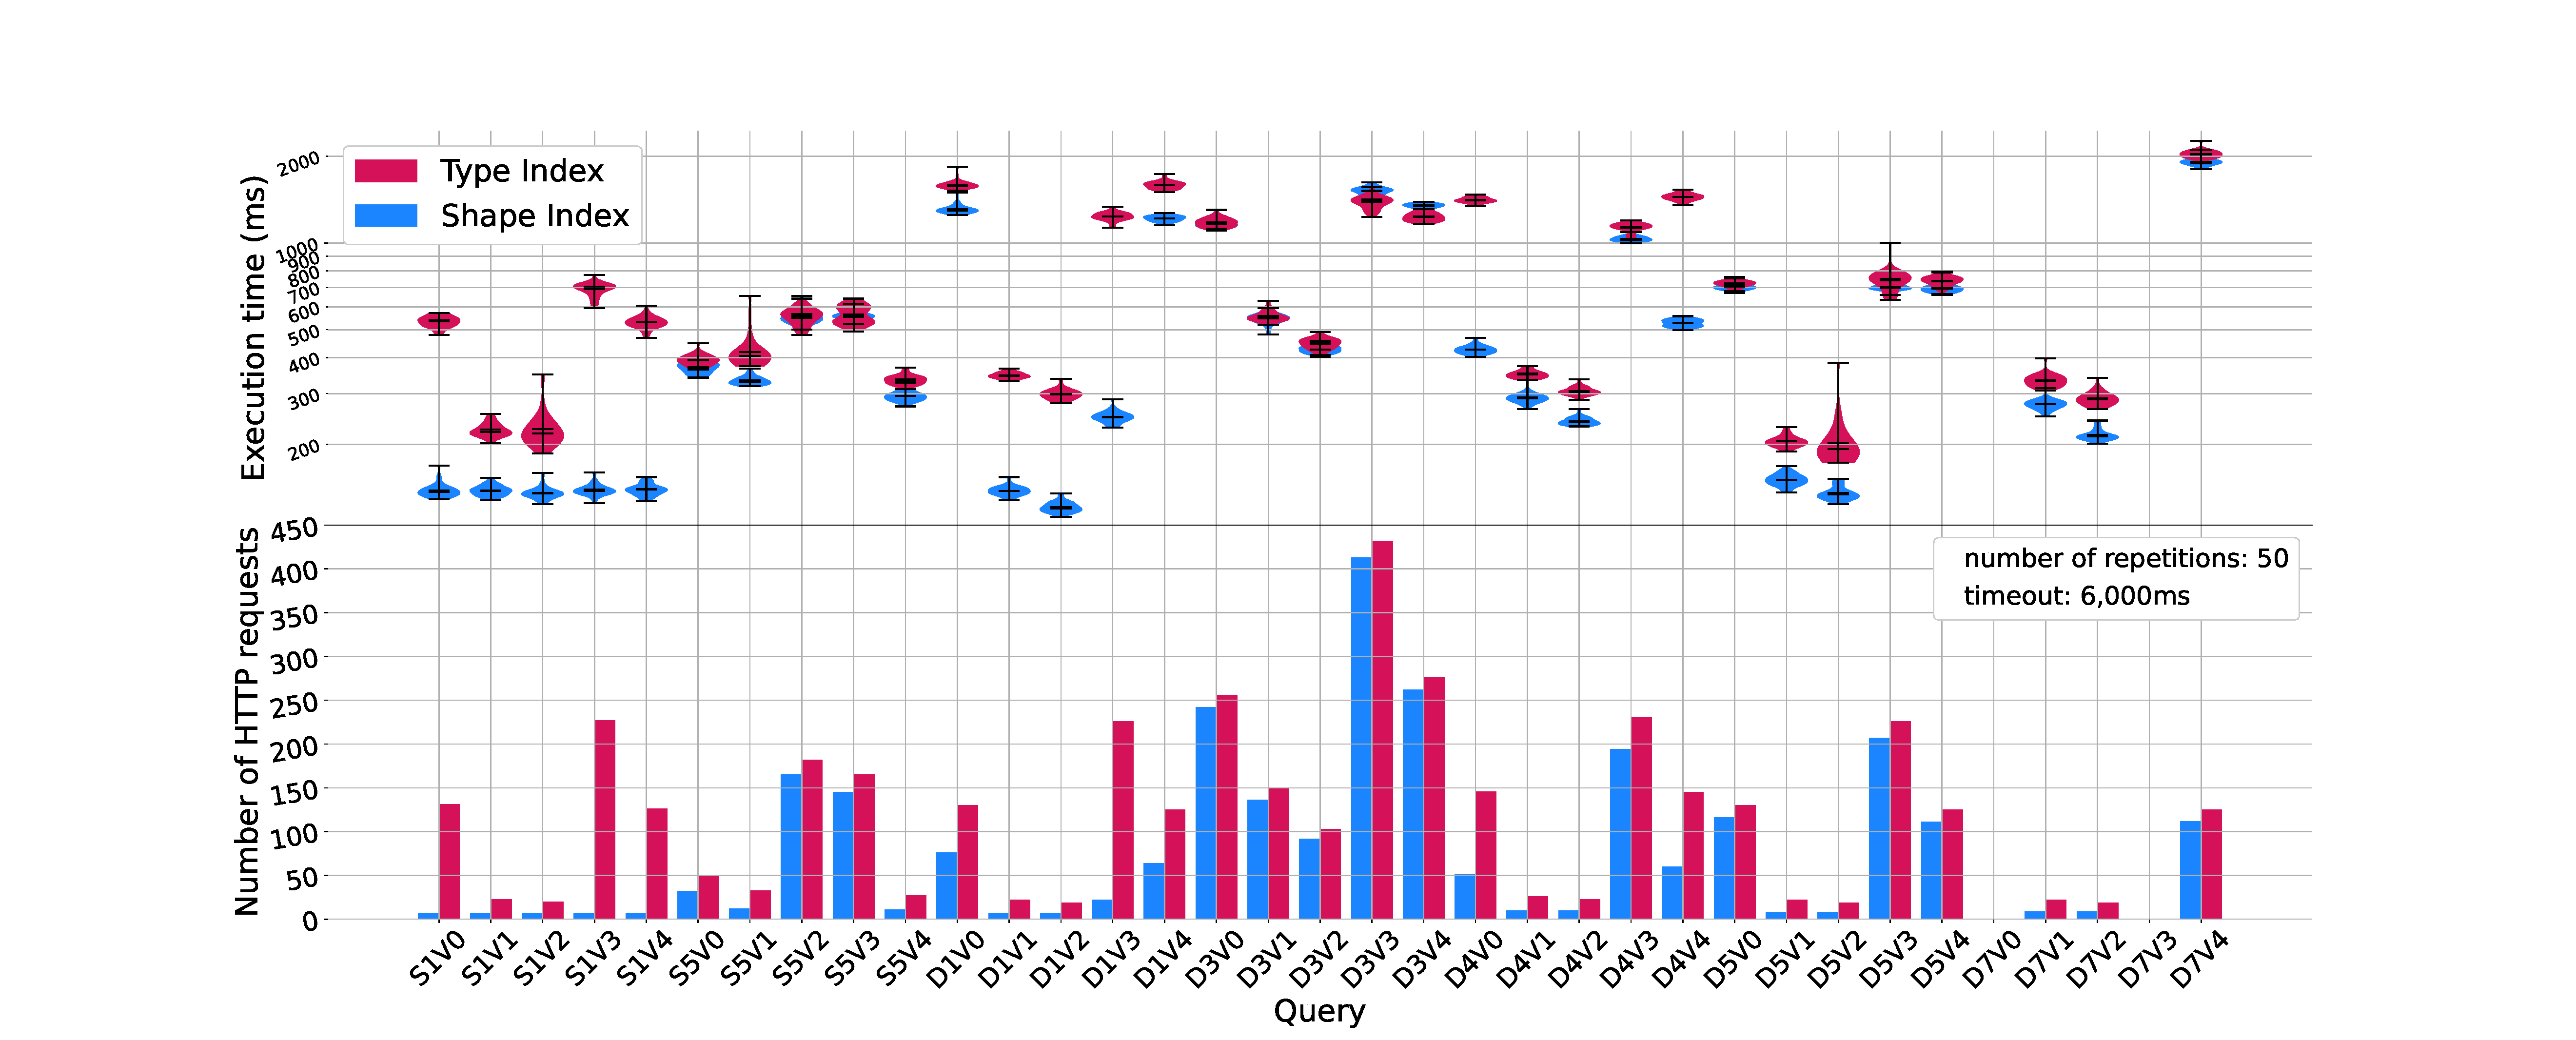
\includegraphics[width=\linewidth]{figure/combined}
  \caption{
  The execution time with shape indexes is consistently lower (up to 80\% with D1V3 and S1V3) or equal to with the type indexes (except for D3V3 and D3V4), and always uses fewer HTTP requests.
  }
  \label{fig:result}
\end{figure}